\documentclass{article}[12pt]
\usepackage{fontspec}   %加這個就可以設定字體
\usepackage{xeCJK}       %讓中英文字體分開設置
\usepackage{indentfirst}
\usepackage{listings}
\usepackage[newfloat]{minted}
\usepackage{float}
\usepackage{graphicx}
\usepackage{caption}
\usepackage{fancyhdr}
\usepackage{hyperref}
\usepackage{amsmath}
\usepackage{multirow}
\usepackage[dvipsnames]{xcolor}
\usepackage{graphicx}
\usepackage{tabularx}
\usepackage{booktabs}
\usepackage{caption}
\usepackage{subcaption}
\usepackage{pifont}
\usepackage{amssymb}

\usepackage[breakable, listings, skins, minted]{tcolorbox}
\usepackage{etoolbox}
\setminted{fontsize=\footnotesize}
\renewtcblisting{minted}{%
    listing engine=minted,
    minted language=python,
    listing only,
    breakable,
    enhanced,
    minted options = {
        linenos, 
        breaklines=true, 
        breakbefore=., 
        % fontsize=\footnotesize, 
        numbersep=2mm
    },
    overlay={%
        \begin{tcbclipinterior}
            \fill[gray!25] (frame.south west) rectangle ([xshift=4mm]frame.north west);
        \end{tcbclipinterior}
    }   
}

\usepackage[
  top=2cm,
  bottom=2cm,
  left=3.5cm,
  right=3.5cm,
  headheight=17pt, % as per the warning by fancyhdr
  includehead,includefoot,
  heightrounded, % to avoid spurious underfull messages
]{geometry} 

\newenvironment{code}{\captionsetup{type=listing}}{}
\SetupFloatingEnvironment{listing}{name=Code}


\title{Introduction to Artificial Intelligence HW4 Report}
\author{110550088 李杰穎}
\date{\today}

\setCJKmainfont{Noto Serif CJK TC}
\setmonofont[Mapping=tex-text]{Consolas}

\XeTeXlinebreaklocale "zh"             %這兩行一定要加,中文才能自動換行
\XeTeXlinebreakskip = 0pt plus 1pt     %這兩行一定要加,中文才能自動換行

\setlength{\parindent}{0em}
\setlength{\parskip}{2em}
\renewcommand{\baselinestretch}{1.25}
\begin{document}

\maketitle

\section{Attention Mechanism of BERT}

\begin{figure}[htbp]
	\centering
	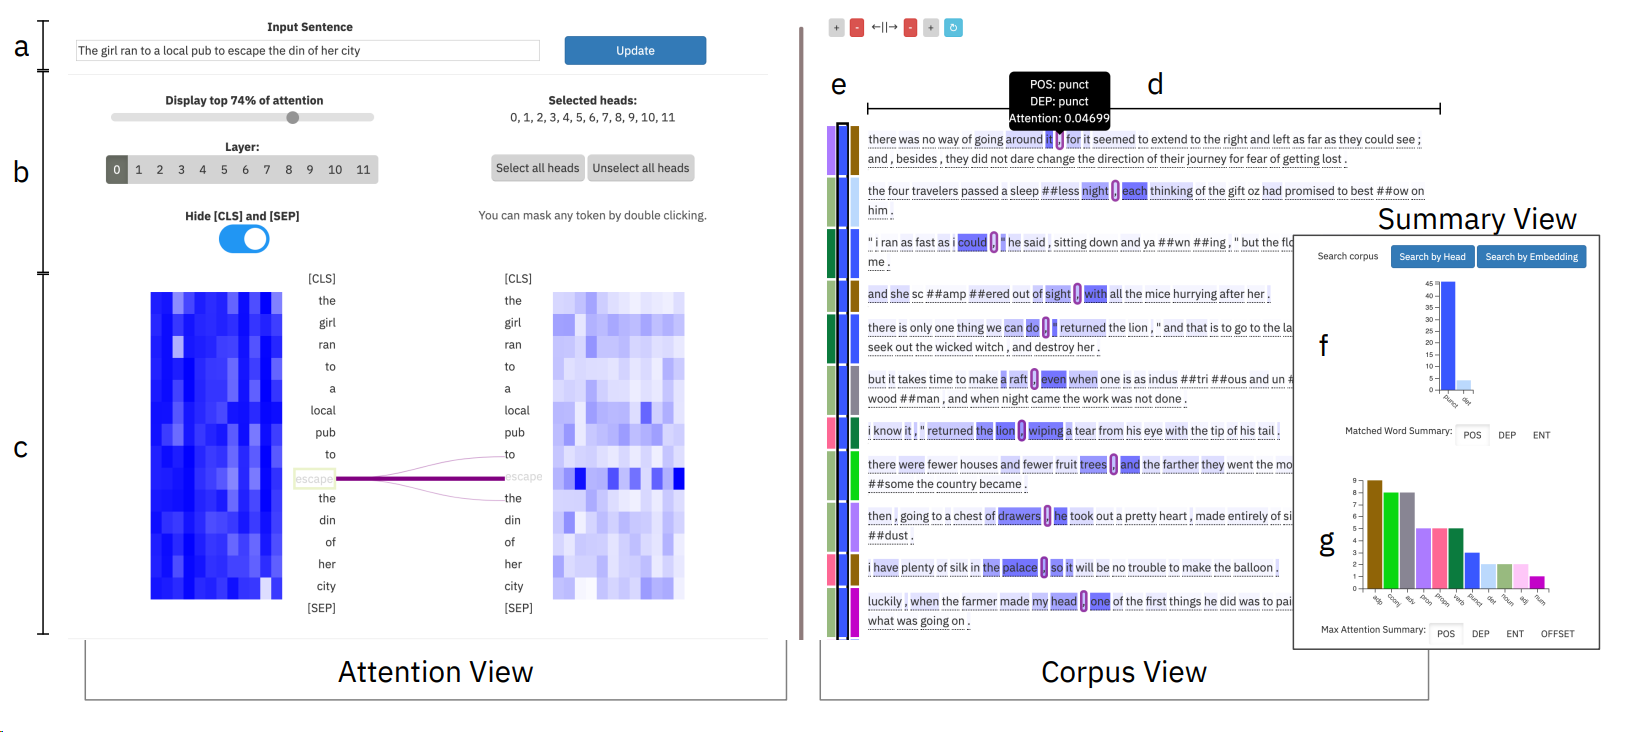
\includegraphics[width=\linewidth]{figure/exbert}
	\caption[]{Screenshot of ExBERT. \footnotemark}
	\label{fig:exbert}
\end{figure}
\footnotetext{From original paper \url{https://arxiv.org/pdf/1910.05276.pdf}}

BERT (Bidirectional Encoder Representation for Transformers) is an NLP model based on transformers. BERT is pre-trained on two tasks, masked language model and next sentence prediction. 

Masked language model is a task that language model needs to predict the masked word. For example, in following sentence, ``The man went to the [MASK] to buy a [MASK] of milk.'' There are two words being masked. BERT needs to predict that those two masked words are ``store'' and ``gallon'', respectively.

Next sentence prediction is a task that model will be given two sentences, let's say sentence A and B. It needs to tell us is B the next sentence of A.

In this section, I will use \href{https://exbert.net}{ExBERT}, a visualizing tool for different variances of BERT, including \texttt{bert-base-cased} and \texttt{distilbert-based-uncased}, to understand the attention mechanisms of BERT.


\subsection{Using BERT as Masked Language Model}

Masked Language Model (MLM) is a task that its input is a sentence with part of words being masked. The goal of language model is to predict the masked words using the context of 
sentence. 

In this section, I will use $\text{BERT}_{\text{base}}$ as language model.

\begin{figure}[htbp]
	\centering
	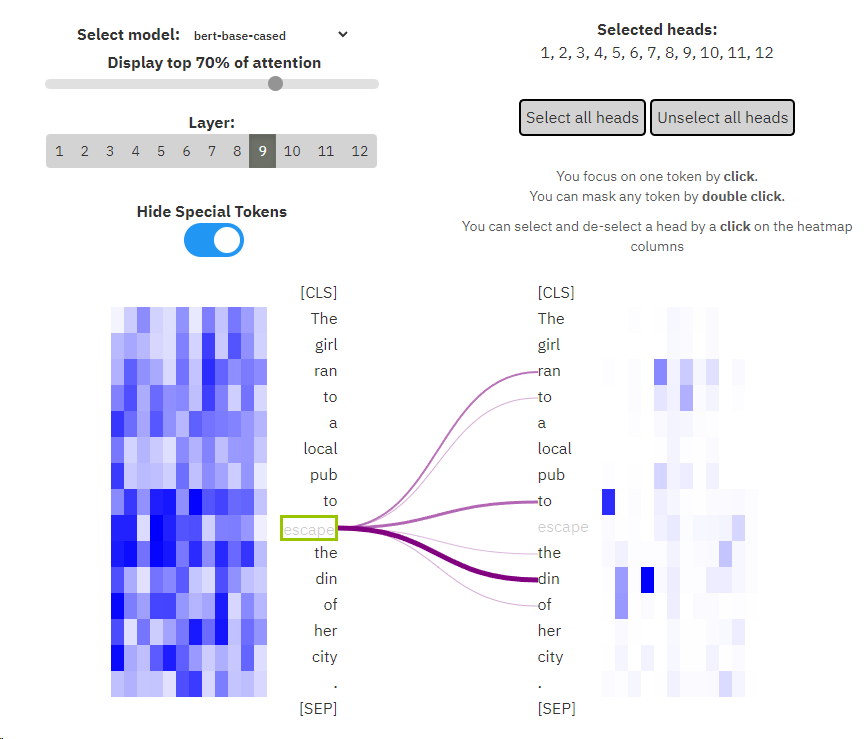
\includegraphics[width=0.7\linewidth]{figure/exbert1}
	\caption{Using the sentence ``The girl ran to a local pub to escape the din of her city.'' and mask the word ``escape''.}
	\label{fig:exbert1}
\end{figure}

As we can see in \autoref{fig:exbert1}, if we mask the word ``escape'' and let BERT predict which word should appear here. In layer 9 of BERT, the words that get attention are ``ran'', ``to'' and ``din''.  These words are exactly the words that is relevance with the masked word ``escape''. This is an example of attention mechanism.


\begin{figure}[htbp]
	\centering
	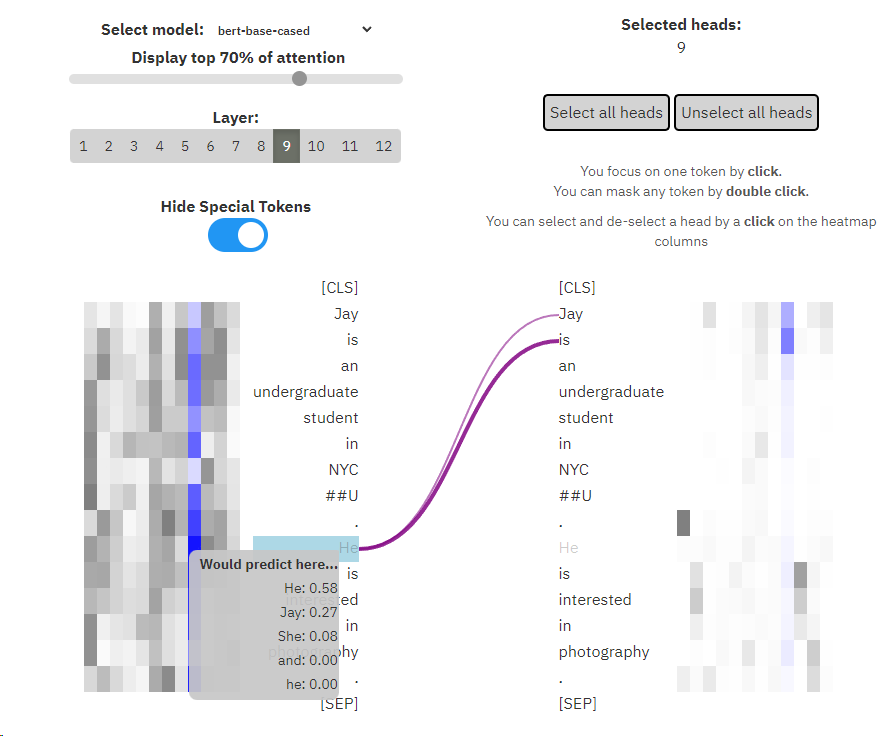
\includegraphics[width=0.7\linewidth]{figure/exbert2}
	\caption{Using the sentence ``Jay is an undergraduate student in NYCU. He is interested in photography.'' and mask the word ``He''.}
	\label{fig:exbert2}
\end{figure}

Another example is shown as \autoref{fig:exbert2}. I mask the subject and see how BERT know what word should be filled in. As a normal human would do. BERT pay its attention on the subject of the first sentence, which is my name ``Jay''. We can also observe that ``He'' has the highest chance to appear in the masked position. This also shows that BERT knows Jay is usually the name of a male.

\begin{figure}[htbp]
	\centering
	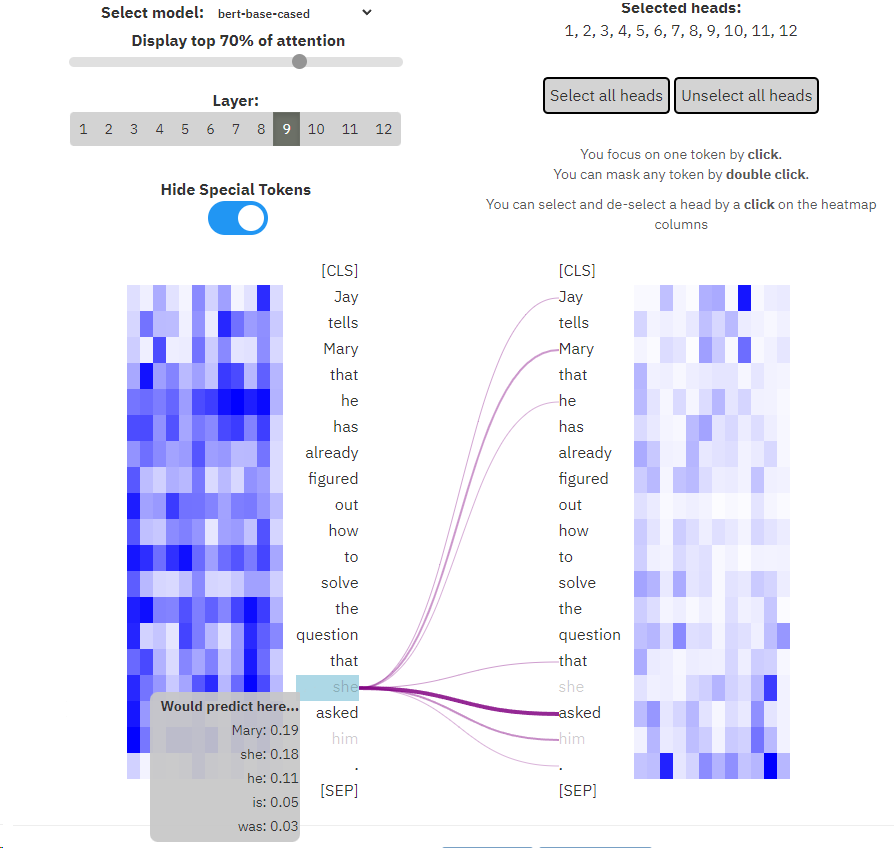
\includegraphics[width=0.7\linewidth]{figure/exbert3}
	\caption{Using the sentence ``Jay tells Mary that he has already figured out how to solve the question that she asked him.'' and mask ``she'' and ``him'' in the second sentence.}
	\label{fig:exbert3}
\end{figure}

The last example is to show that BERT is able to know that who does a specific pronoun refer to. As we can see in the \autoref{fig:exbert3}, BERT pays its attention at ``Mary" when it predict the masked word, instead of ``Jay''. This shows that BERT can analysis the grammar structure in the sentence and know which word should be paid attention at.

In conclusion, the examples above show that how attention mechanism work in BERT. And indeed, this mechanism helps BERT perform better compared with other methods like n-gram model or ELMo.

\section{Comparison of BERT and DistilBERT}

DistilBERT is smaller version of BERT. The basic idea of DistilBERT is to use a light-weight model architecture to ``mimic'' the behavior of the original BERT. The author of DistilBERT claimed that this method can ``reduce the size of a BERT by 40\%, while retaining 97\% of its language understanding capabilities and being 60\% faster.''\footnote{From abstract of original paper. \url{https://arxiv.org/abs/1910.01108}}

In ExBERT, we can use both \texttt{bert-base-cased} and \texttt{distilbert-base-uncased}. Thus, we will also use ExBERT to compare these two model.

To compare DistilBERT with BERT. I use the same three sentences as in previous section and mask same words. Below are the experiments results. Noticed that these results are all from layer 3 of DistilBERT. This is because after some observations, I think this is layer that DistilBERT pay attention to the context of sentence. Other layers are paying attention to either the previous word or the next word or the [CLS] tag.

\begin{figure}[htbp]
	\centering
	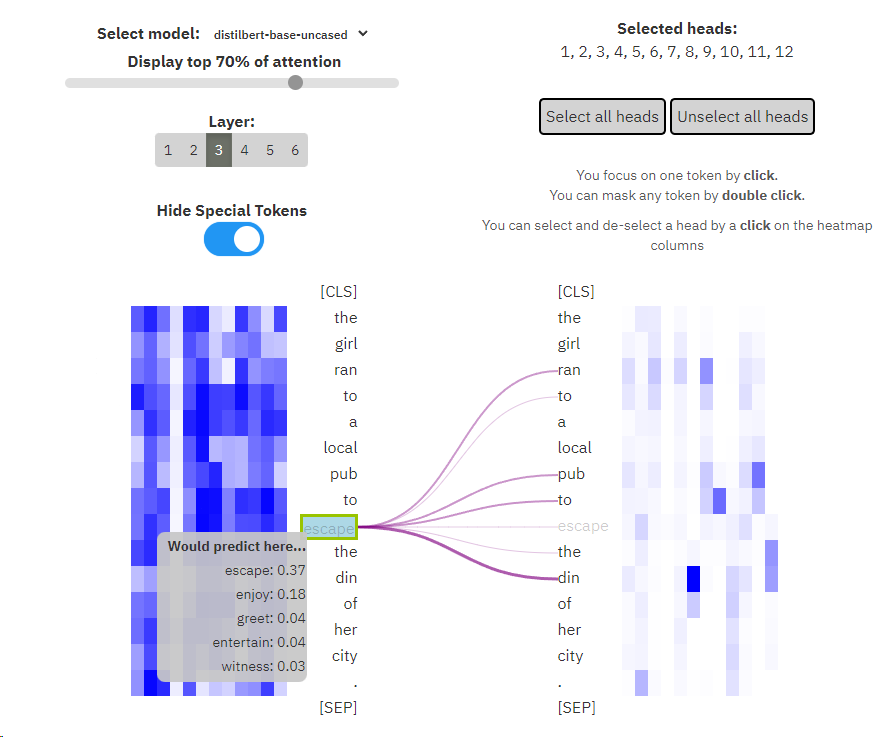
\includegraphics[width=0.7\linewidth]{figure/exbert-distil1}
	\caption{Using the sentence ``The girl ran to a local pub to escape the din of her city.'' and mask the word ``escape''.}
	\label{fig:exbert-distil1}
\end{figure}

As we can see in \autoref{fig:exbert-distil1}, DistilBERT is able to predict correctly, and the words it pays attention to is similar to those BERT pays attention to. This shows that DistilBERT learn some ``knowledges'' from the original BERT.

\begin{figure}[htbp]
	\centering
	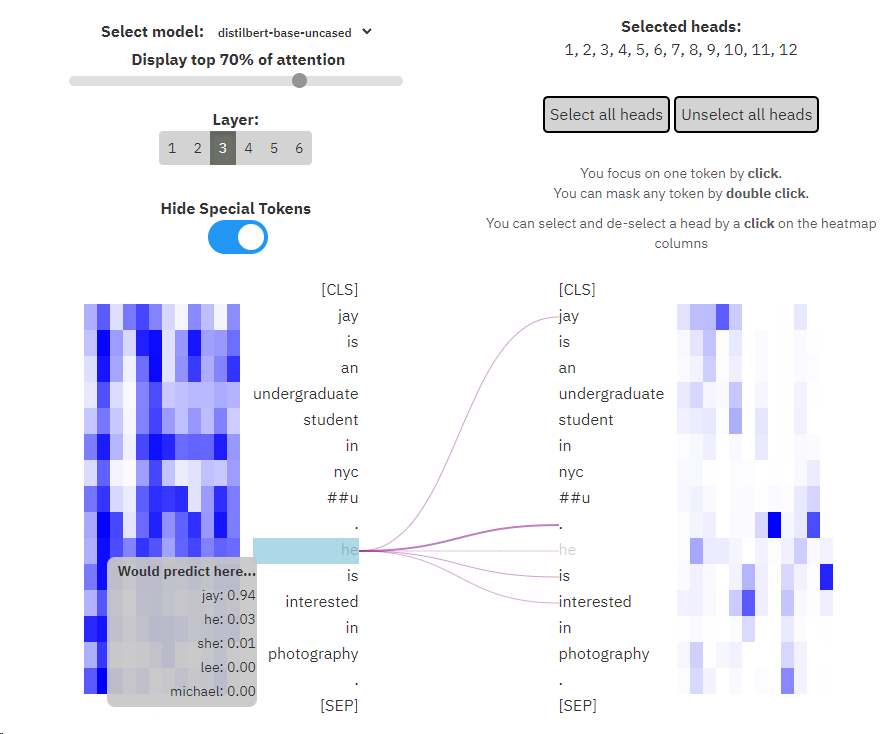
\includegraphics[width=0.7\linewidth]{figure/exbert-distil2}
	\caption{Using the sentence ``Jay is an undergraduate student in NYCU. He is interested in photography.'' and mask the word ``He''.}
	\label{fig:exbert-distil2}
\end{figure}


\begin{figure}[htbp]
	\centering
	\begin{subfigure}[b]{0.45\textwidth}
		\centering
		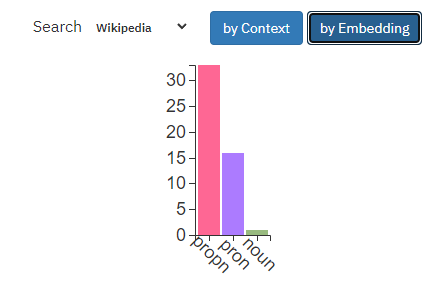
\includegraphics[width=\textwidth]{figure/exbert-distil4}
		\caption{DistilBERT}
		\label{fig:exbert-distilbert-embedding}
	\end{subfigure}
	\hfill
	\begin{subfigure}[b]{0.45\textwidth}
		\centering
		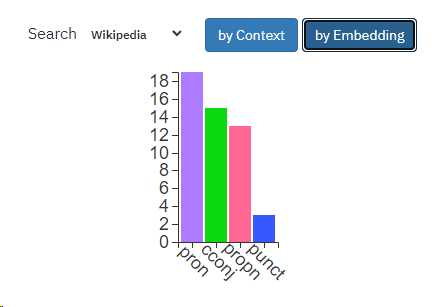
\includegraphics[width=\textwidth]{figure/exbert-distil5}
		\caption{BERT}
		\label{fig:exbert-bert-embedding}
	\end{subfigure}
	\caption{The matched word summary of the sentence ``Jay is an undergraduate student in NYCU. He is interested in photography.'' and mask the word ``He''.}
\end{figure}


\begin{figure}[htbp]
	\centering
	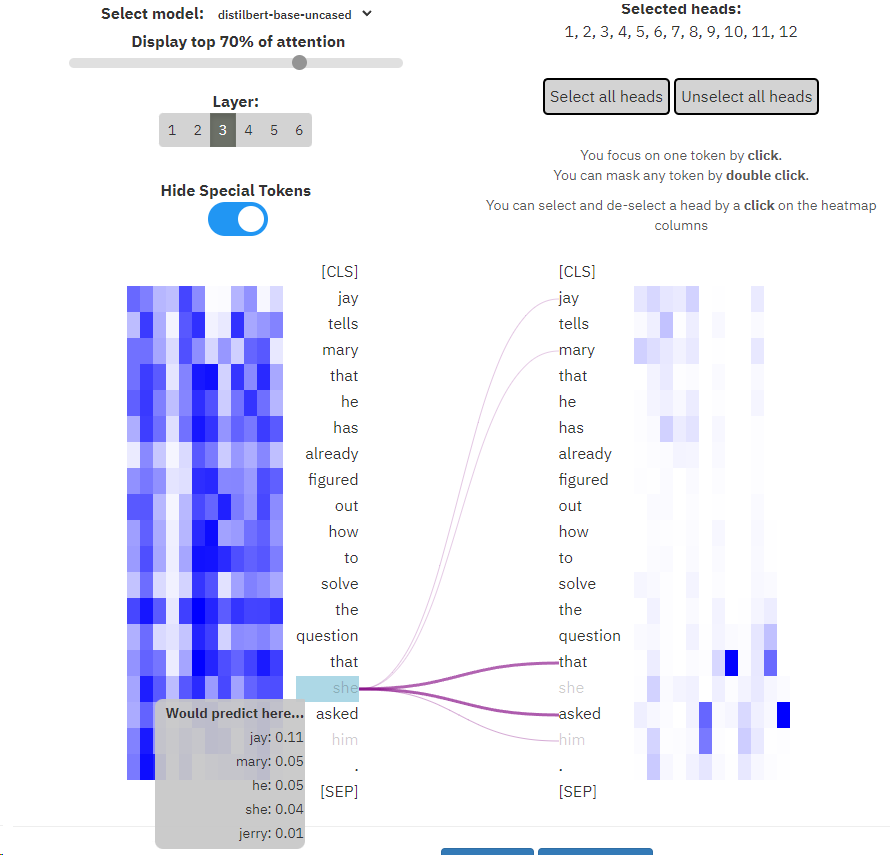
\includegraphics[width=0.7\linewidth]{figure/exbert-distil3}
	\caption{Using the sentence ``Jay tells Mary that he has already figured out how to solve the question that she asked him.'' and mask ``she'' and ``him'' in the second sentence.}
	\label{fig:exbert-distil3}
\end{figure}

But if we look at more complicate examples, like sentences in \autoref{fig:exbert-distil2} and \autoref{fig:exbert-distil3}, DistilBERT can't predict the masked word as well as original BERT can do.

Let's first look at \autoref{fig:exbert-distil2}. DistilBERT can predict that the masked word can be the name ``Jay'' or ``He''. Although both of these is correct answer and model knows that Jay is a male name. But the better answer is ``He'', which is closer to daily English usage. But DistilBERT only has 3\% of probability to fill ``He'' here. This shows that DistilBERT perform worse than original BERT. 

Furthermore, we can also use the ``by Embedding'' button to see the matched word. \autoref{fig:exbert-distilbert-embedding} shows that the matched word summary in the last layer of DistilBERT. In contrast, \autoref{fig:exbert-bert-embedding} shows that the matched word summary in the last layer of BERT. We can see that BERT matched more pronoun than DistilBERT does, which is a better matched compared with proper noun. This also shows the difference between BERT and DistilBERT.

\autoref{fig:exbert-distil3} is the last example. Compared with the result shown in \autoref{fig:exbert3}, DistilBERT's prediction is completely wrong, the most possible word is ``Jay'', which is the last word to be filled in. This example shows that there has a significant performance difference between BERT and DistilBERT.

In conclusion, although DistilBERT can predict words correctly in some simple sentences, but if the sentences are too complicate, DistilBERT may not perform very well.

\section{Explainable AI: LIME and SHAP}

Nowadays, people have trained lots of AI models to do various of tasks. But most of these models are black boxes, we don't know how machine makes its decision. This makes us hard to trust the prediction of machine. Even worse, if the models make some wrong decision, it's nearly impossible to debug those AI models. Therefore, we need to conceive methods to explain behavior of AI models. In this section, I will discuss two methods that can explain AI models. One of them is local interpretable model-agnostic explanations (LIME) and another is shapley additive explanations (SHAP).

\subsection{Local Interpretable Model-agnostic Explanations (LIME)}

LIME is an method to explain AI model. Its name clearly shows its properties.

\begin{enumerate}
	\item \textbf{Local}: LIME explain the given prediction locally.
	\item \textbf{Interpretable}: The explanation given by LIME is easy enough for human to understand.
	\item \textbf{Model-agnostic}: Treat the model as a black box so that LIME works on every model.
\end{enumerate}

Given a prediction we want to explain, LIME first creates a datasets by perturbed the given input. Then it uses this datasets to train a simple (often a linear classifier) and explainable classifier. The performance of this classifier need to be good enough on the new datasets. In this way, we can achieved the so-called ``local fidelity''. \autoref{fig:lime-classifier} illustrates above procedures. $g(z')$ is the classifier we want to train.

\begin{figure}[htbp]
	\centering
	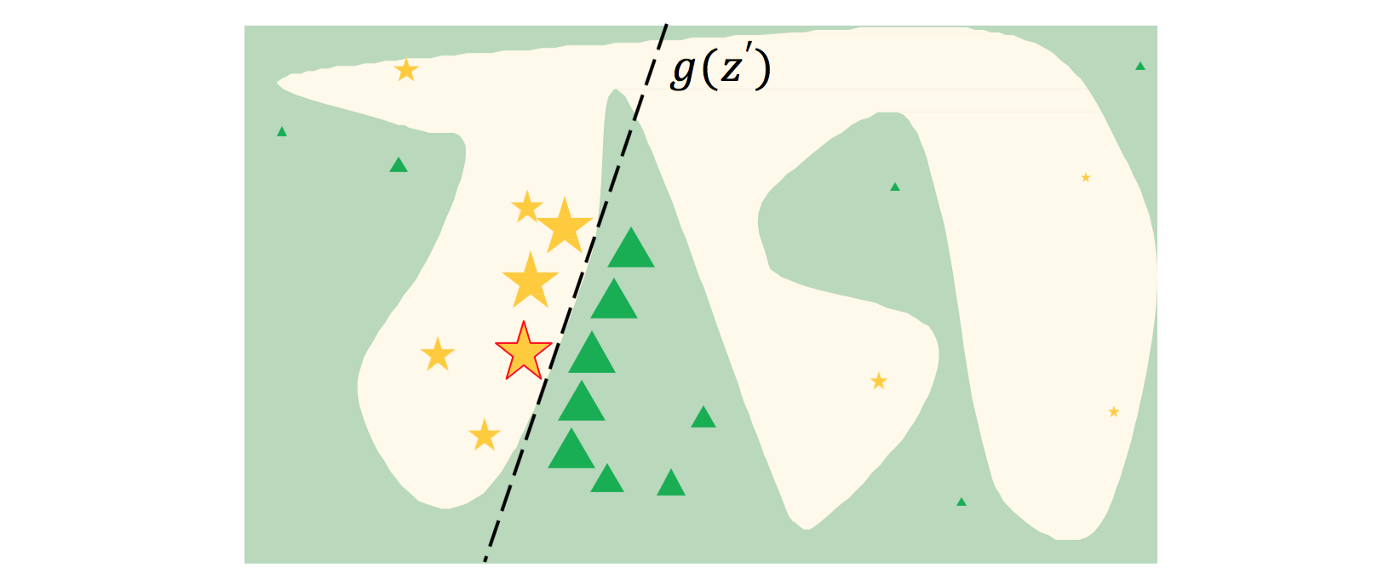
\includegraphics[width=0.7\linewidth]{figure/lime-classifier}
	\caption[]{A simple classifier.\footnotemark}
	\label{fig:lime-classifier}
\end{figure}
\footnotetext{From \url{https://reurl.cc/3o4YE8}}

We can noticed that LIME only works on a single prediction. We can't get a global explanation using LIME. On the contrast, the next method I will introduce works both on local and global explanation.

\subsection{Shapley Additive Explanations (SHAP)}

SHAP is an method based on Shapley value. Shapley value is first proposed by an American mathematician Lloyd Stowell Shapley. Shapley value can be used to compute the contribution to the final output of model for a given feature. The following equation is for computing the Shapley value for a given feature $j$.

\begin{equation}
\phi_{i}=\sum_{S \subseteq F \backslash\{i\}} \frac{|S| !(|F|-|S|-1) !}{|F| !}\left[f_{S \cup\{i\}}\left(x_{S \cup\{i\}}\right)-f_{S}\left(x_{S}\right)\right]
\end{equation}

Where $F$ is all the features used to build the model. $f_{S}(x_{S})$ is the output of the model trained with feature set $S$.\footnote{For detailed explanation, please refer to the original paper or this article. \url{https://papers.nips.cc/paper/2017/hash/8a20a8621978632d76c43dfd28b67767-Abstract.html}}

We can also noticed that SHAP deals with features, it can also give the global explanation. In the next subsection, I will compare the local explanation given by LIME and SHAP. And I will also show the global explanation given by SHAP using the IMDB datasets.

\subsection{Explanations Given by LIME and SHAP}

Before using the sentences from IMDB Datasets to test LIME and SHAP. Let's first look at some simpler sentences. And also, I will test two models given by TAs, which are \texttt{distilbert-base-uncased} and \texttt{prajjwal1/bert-small}. And because these two models are trained on IMDB datasets to classify the sentiment of given movie review. Therefore, the sentences that I will test in experiments all express strong sentiments.

\subsubsection{Using Simple Sentences}

I will use four sentences 

\begin{enumerate}
	\item It was a fantastic performance!
	\item That is a terrible movie.
	\item This movie is a must-see.
	\item This movie really brings art to a new level.	
\end{enumerate}

Below is the explanation of four sentences given by LIME and SHAP. Model used here is \texttt{distilbert-base-uncased}.

\begin{figure}[htbp]
	\centering
	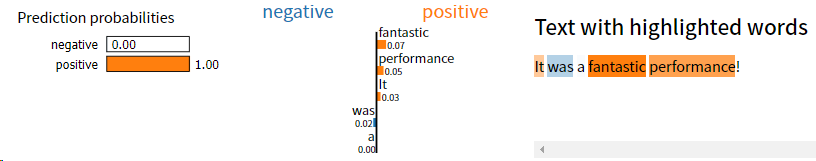
\includegraphics[width=\linewidth]{figure/lime-simple-1}
	\caption{The explanation of first sentence given by LIME.}
	\label{fig:lime-simple-1}
\end{figure}

\begin{figure}[htbp]
	\centering
	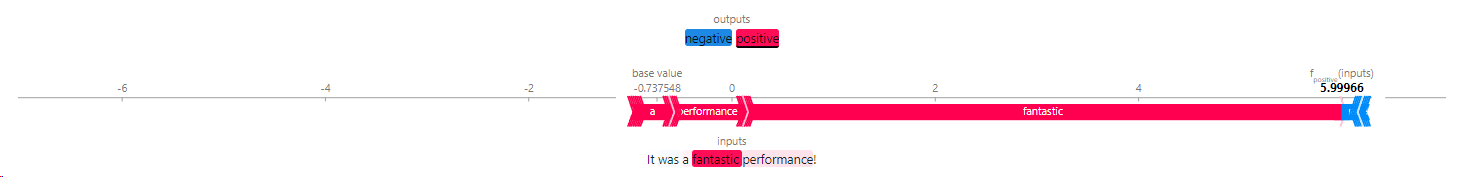
\includegraphics[width=\linewidth]{figure/shap-simple-1}
	\caption{The explanation of first sentence given by SHAP.}
	\label{fig:shap-simple-1}
\end{figure}

\begin{figure}[htbp]
	\centering
	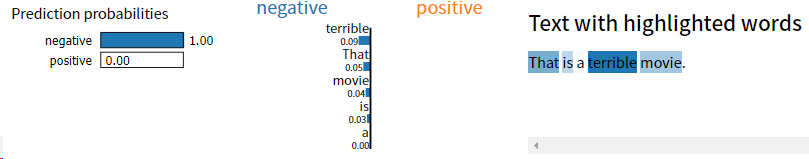
\includegraphics[width=\linewidth]{figure/lime-simple-2}
	\caption{The explanation of second sentence given by LIME.}
	\label{fig:lime-simple-2}
\end{figure}

\begin{figure}[htbp]
	\centering
	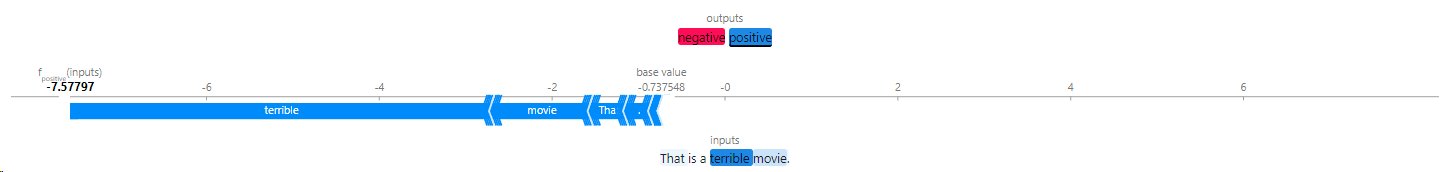
\includegraphics[width=\linewidth]{figure/shap-simple-2}
	\caption{The explanation of second sentence given by SHAP.}
	\label{fig:shap-simple-2}
\end{figure}

\begin{figure}[htbp]
	\centering
	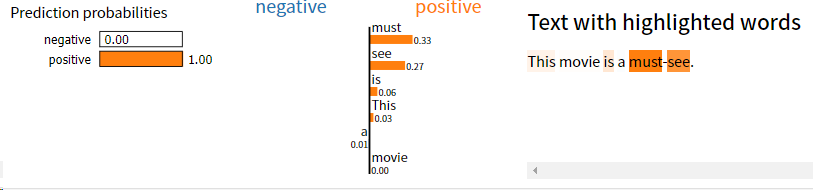
\includegraphics[width=\linewidth]{figure/lime-simple-3}
	\caption{The explanation of third sentence given by LIME.}
	\label{fig:lime-simple-3}
\end{figure}

\begin{figure}[htbp]
	\centering
	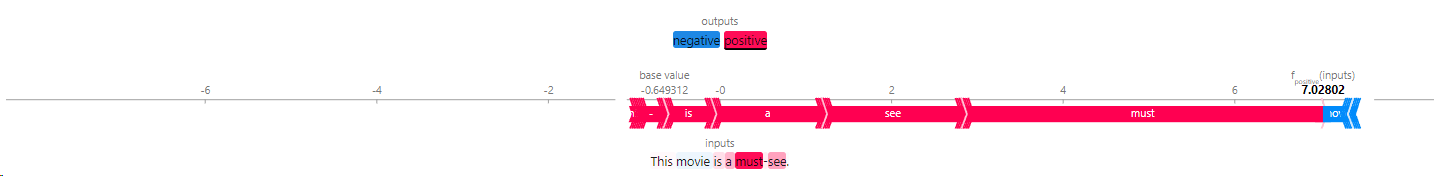
\includegraphics[width=\linewidth]{figure/shap-simple-3}
	\caption{The explanation of third sentence given by SHAP.}
	\label{fig:shap-simple-3}
\end{figure}

\begin{figure}[htbp]
	\centering
	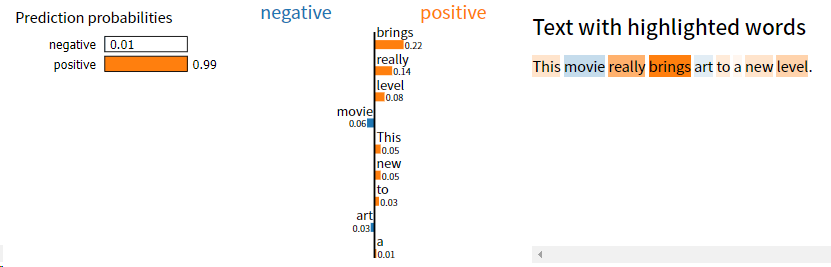
\includegraphics[width=\linewidth]{figure/lime-simple-4}
	\caption{The explanation of fourth sentence given by LIME.}
	\label{fig:lime-simple-4}
\end{figure}

\begin{figure}[htbp]
	\centering
	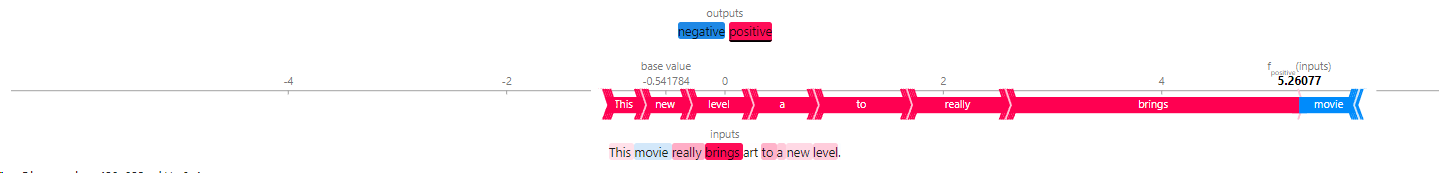
\includegraphics[width=\linewidth]{figure/shap-simple-4}
	\caption{The explanation of fourth sentence given by SHAP.}
	\label{fig:shap-simple-4}
\end{figure}

As we can see from \autoref{fig:lime-simple-1} to \autoref{fig:shap-simple-4}, both LIME and SHAP can explain the prediction very well. Both method can give us the contribution of each word to the result. Even a harder sentence like the third and fourth sentences (\autoref{fig:lime-simple-3} to \autoref{fig:shap-simple-4}), which doesn't mention any sentimental word, both methods can know that ``brings art to a new level'' and ``must-see'' has positive meaning and is important to the final prediction.

\subsubsection{Using Sentences from IMDB Datasets}

In this section, I will use the reviews in test set of IMDB Datasets. I've picked four reviews, I will list them below. The first and second reviews are positive samples and rest of them are negative samples.

\begin{enumerate}
	\footnotesize
	\item I bought the DVD a long time ago and finally got around to watching it.I really enjoyed watching this film as you don't get the chance to see many of the more serious better quality bollywood films like this. Very well done and but I would say you need to pay attention to what is going on as it is easy to get lost. When you start watching the movie, don't do anything else! I would actually advise people to read all the reviews here...including the ones with spoilers, before watching the movie. Raima Sen gave her first great performance that I have seen. Aishwarya was easily at her best. All performances were strong, directing and cinematography...go watch it!
	\item A ghost story on a typical Turkish high school with nice sound and visual effects. Taylan biraderler(taylan brothers) had made their first shots on a tv-show a couple of years ago, as far as i know. That was kind of a Turkish X-Files, they had very nice stories but lacked on visual effects. This time it seems they had what they needed and used them well. This movie will make you laugh that's for sure, and as well it might have you scared. It has a nice plot and some young, bright actors in it. If you are a high school student in Turkey you will find so many things about you here. There are many clues in the movie about its story and ending, some you understand at the moment, some will make sense afterwords, the dialogs were written very cleverly. So these make the movie one of the best Turk movies made in the last years. Do not forget, this movie is the first of its kind in the Turkish film industry.
	\item This movie is so unreal. French movies like these are just waste of time. Why watch this movie? Even, I did not know..why. What? The well known sex scene of half-siblings? Although the sex scene is so real and explicit, but the story it is based upon is so unreal. What is the use of it, then? Can you find easily in life, half sibling doing such things?<br /><br />Did I learn something from this movie? Yeah: some people are just so fond of wasting time making such movies, such stories, such non-sense. But for those who like nihilism, nothingness in life, or simply a life without hope, then there you are.. you've got to see this movie.<br /><br />Only one worth adoring, though: CATHERINE DENEUVE. She's such a strikingly beautiful woman.
	\item I saw this with high expectations. Come on, it is Akshay Kumar, Govinda, and Paresh Rawal, who are all amazing at their comedy, I was really hoping for a laugh riot. Sadly, that is not what I got at all...<br /><br />Unfortunately, nothing in this movie really made me laugh out loud. There were times when I chuckled at one or two things, but nothing really made me laugh. In short, it was badly attempted comedy, and in a way, a bit of a Hera Pheri wannabe.<br /><br />Out of the three main guys, I think Paresh Rawal's role was the most powerful. It wasn't the biggest role, but it certainly stood out more than Govinda or Akshay. Their performances were okay I guess. Nothing special, just mediocre. Though Govinda stole the limelight from Akshay in more than a few scenes. Lara Dutta and Tanushree Dutta also make appearances in this film, and both of them were pretty bad. Lara's role did not move me, or make me laugh, and Tanushree Dutta's character just got on my nerves! The music seems to be the only good thing about Bhagam Bhag. My favourite song is "Tere Bin", followed by "Afreen", which I really liked. "Signal" and the title song "Bhagam Bhag" are also worth a listen.<br /><br />You either will like it or you won't. And judging by the poor comedy and lack of direction, I don't think you will.
	
\end{enumerate}

Below is the explanation of four reviews given by LIME and SHAP. Model used here is also \texttt{distilbert-base-uncased}. 

\begin{figure}[htbp]
	\centering
	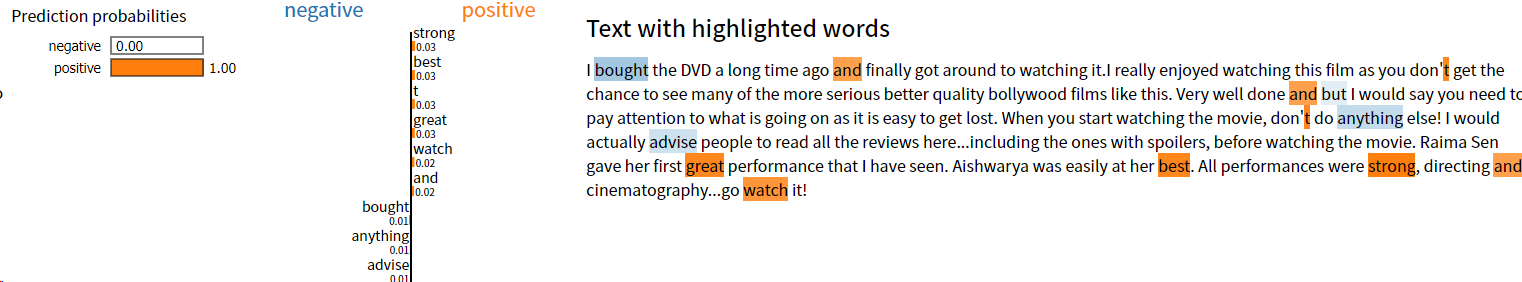
\includegraphics[width=\linewidth]{figure/lime-imdb-1}
	\caption{The explanation of first review given by LIME.}
	\label{fig:lime-imdb-1}
\end{figure}

\begin{figure}[htbp]
	\centering
	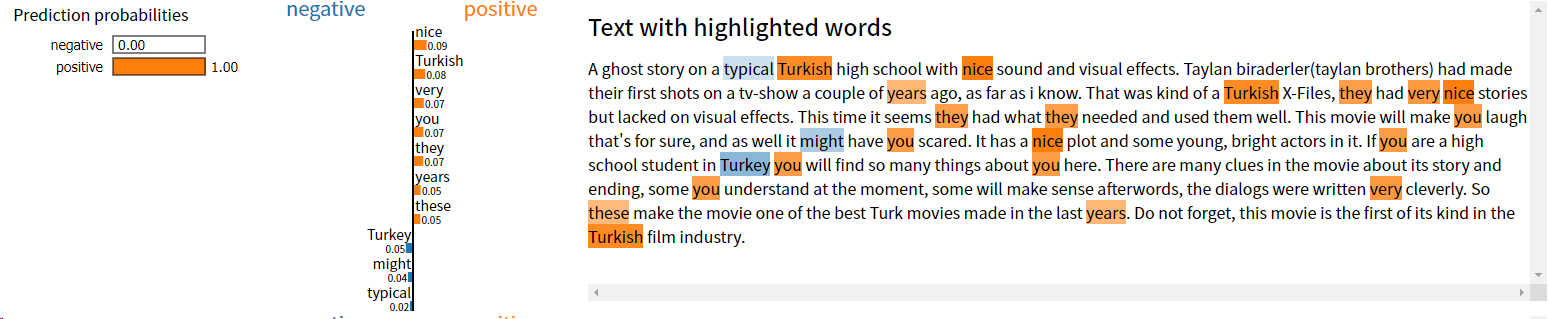
\includegraphics[width=\linewidth]{figure/lime-imdb-2}
	\caption{The explanation of second review given by LIME.}
	\label{fig:lime-imdb-2}
\end{figure}

\begin{figure}[htbp]
	\centering
	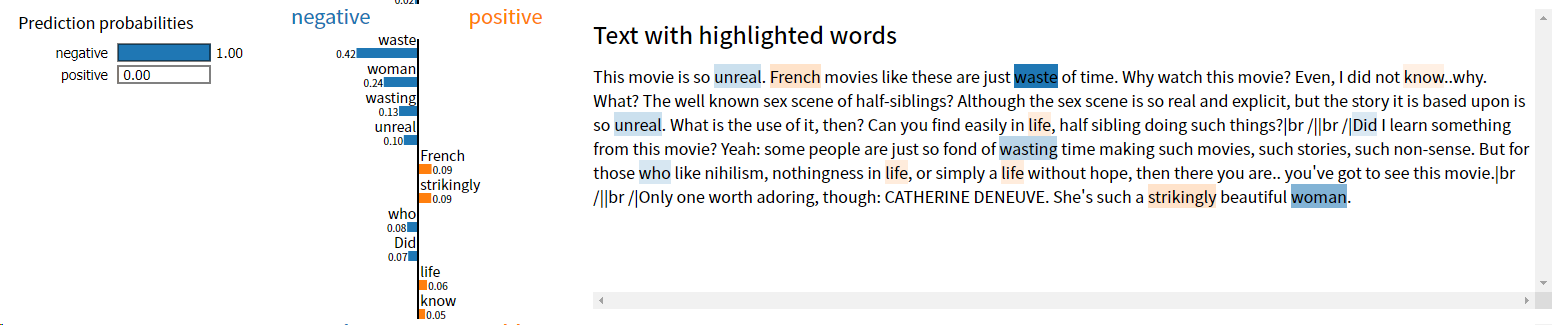
\includegraphics[width=\linewidth]{figure/lime-imdb-3}
	\caption{The explanation of third review given by LIME.}
	\label{fig:lime-imdb-3}
\end{figure}

\begin{figure}[htbp]
	\centering
	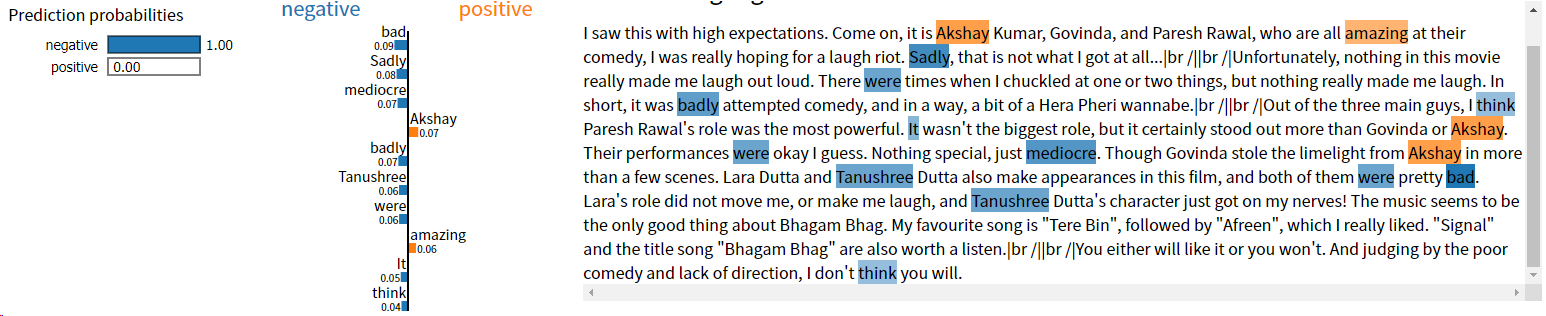
\includegraphics[width=\linewidth]{figure/lime-imdb-4}
	\caption{The explanation of fourth review given by LIME.}
	\label{fig:lime-imdb-4}
\end{figure}

\begin{figure}[htbp]
	\centering
	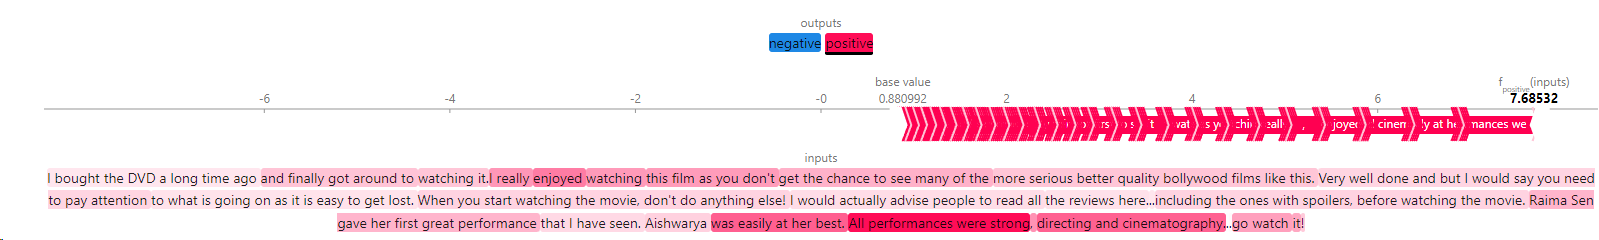
\includegraphics[width=\linewidth]{figure/shap-imdb-1}
	\caption{The explanation of first review given by SHAP.}
	\label{fig:shap-imdb-1}
\end{figure}

\begin{figure}[htbp]
	\centering
	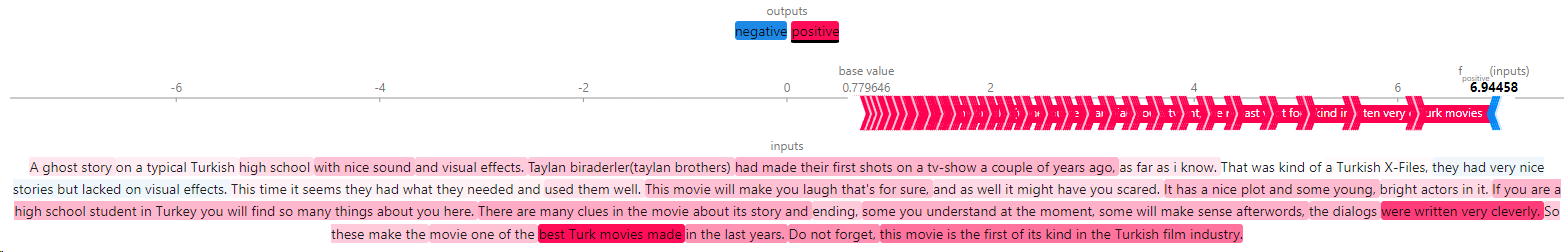
\includegraphics[width=\linewidth]{figure/shap-imdb-2}
	\caption{The explanation of second review given by SHAP.}
	\label{fig:shap-imdb-2}
\end{figure}

\begin{figure}[htbp]
	\centering
	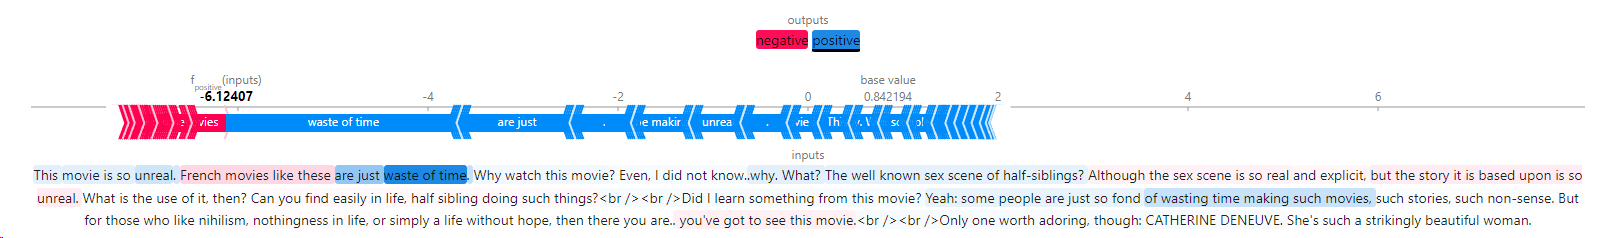
\includegraphics[width=\linewidth]{figure/shap-imdb-3}
	\caption{The explanation of third review given by SHAP.}
	\label{fig:shap-imdb-3}
\end{figure}

\begin{figure}[htbp]
	\centering
	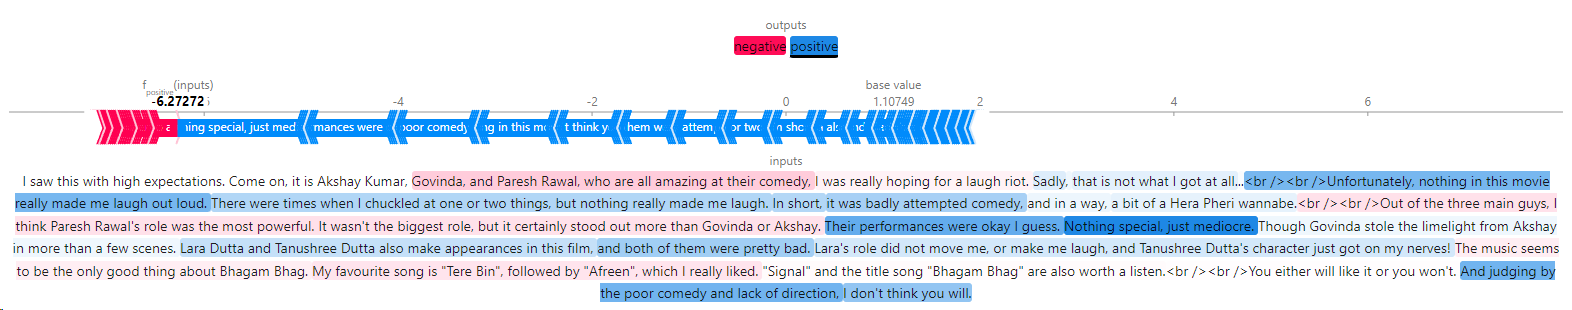
\includegraphics[width=\linewidth]{figure/shap-imdb-4}
	\caption{The explanation of fourth review given by SHAP.}
	\label{fig:shap-imdb-4}
\end{figure}

As we can observe in \autoref{fig:lime-imdb-1} to \autoref{fig:shap-imdb-4}. Although LIME and SHAP both can explain short sentence really well. However, when it comes to the explanation of long sentences like movie reviews in IMDB datasets, explanation given by LIME are worse than those given by SHAP. LIME can only marked some single words instead of whole sentence like SHAP give us. To be worse, some words that LIME marked are unreasonable. For example, like in \autoref{fig:lime-imdb-3}, LIME marked the last word ``woman'', and said that it's contribution to the negative prediction is second high among all the words, which is absolutely wrong. On the contrary, \autoref{fig:shap-imdb-3} shows the explanation of third review given by SHAP. As we can see, this explanation is way better than LIME gives. It marks the word by phrases and those which get high Shapley value are indeed the main reason why this review is negative. It can also mark the positive part of a negative review. Therefore, I think SHAP is a better explanation techniques than LIME when it comes to sentimental classification.

And I think the reason why LIME's explanation of long sentences is worse than short sentence is mainly because LIME treats every word in the review as a feature. Therefore, if there are too many features (like in movie review), it's very hard to generate a stable perturbed datasets. And also, we can't train a simple classifier to approximate the original model.

Another disadvantage of LIME is that LIME generates the perturbed datasets randomly. Therefore, the explanation given by LIME is different. \autoref{fig:lime-imdb-random} shows this effect. I input same review in \autoref{fig:lime-imdb-1}, but the final explanation is completely different.

\begin{figure}[htbp]
	\centering
	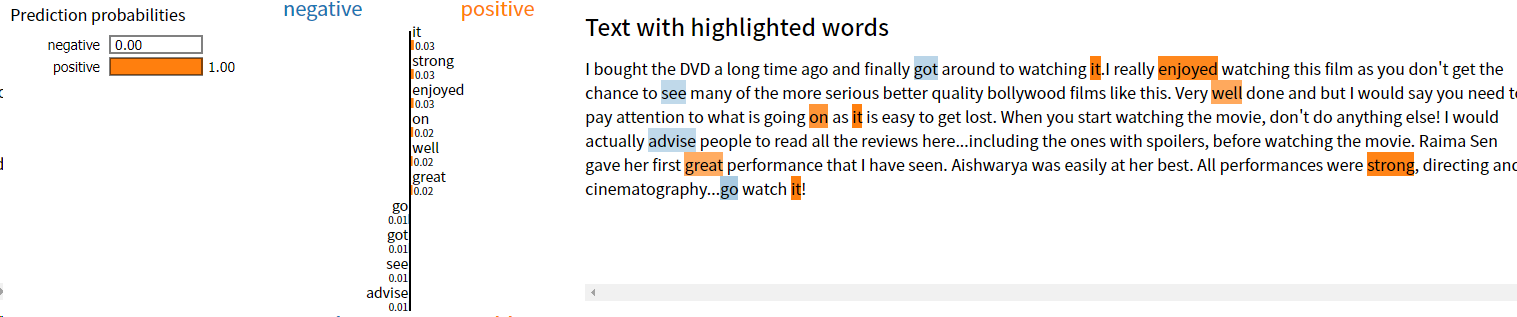
\includegraphics[width=\linewidth]{figure/lime-imdb-random}
	\caption{The randomness in explanation give by LIME.}
	\label{fig:lime-imdb-random}
\end{figure}

In conclusion, I personally think that SHAP is a better explanation technique than LIME.


\section{Other Explanation Technique}

\section{Attack NLP Model}

\section{Encountered Problems}


\end{document}